% !TEX TS-program = pdflatex
% !TEX encoding = UTF-8 Unicode
% !TEX ROOT = main.tex
\section{Gebäudeplan Kirchhoff-Institut für Physik (KIP)}
\begin{figure}[H]
\centering
\begin{subfigure}[h]{0.62\textwidth}
\centering
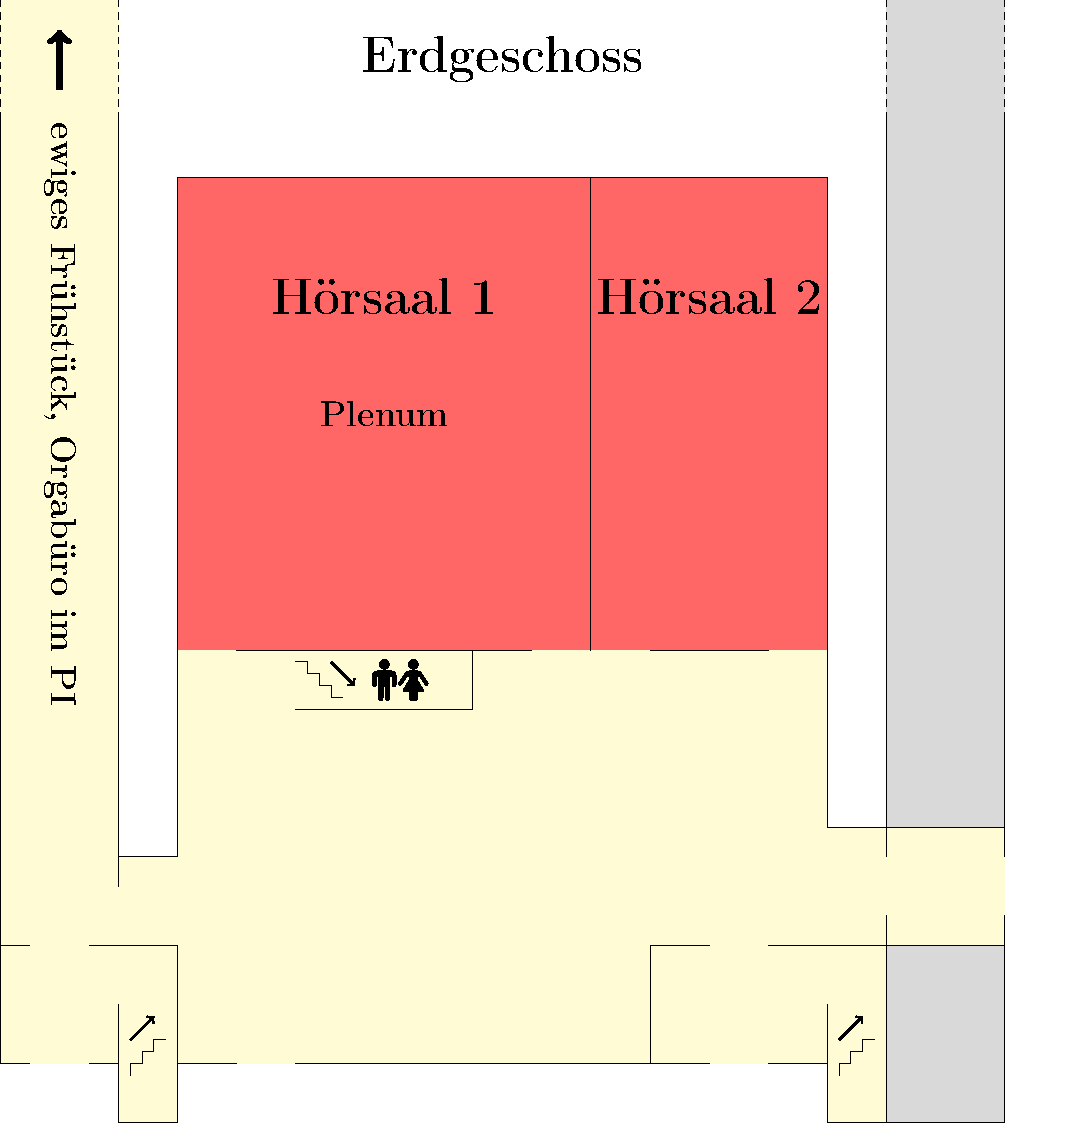
\includegraphics[width=\linewidth]{raumplan/eg}
\vspace*{5mm}
\end{subfigure}
\begin{subfigure}[h]{0.62\textwidth}
\centering
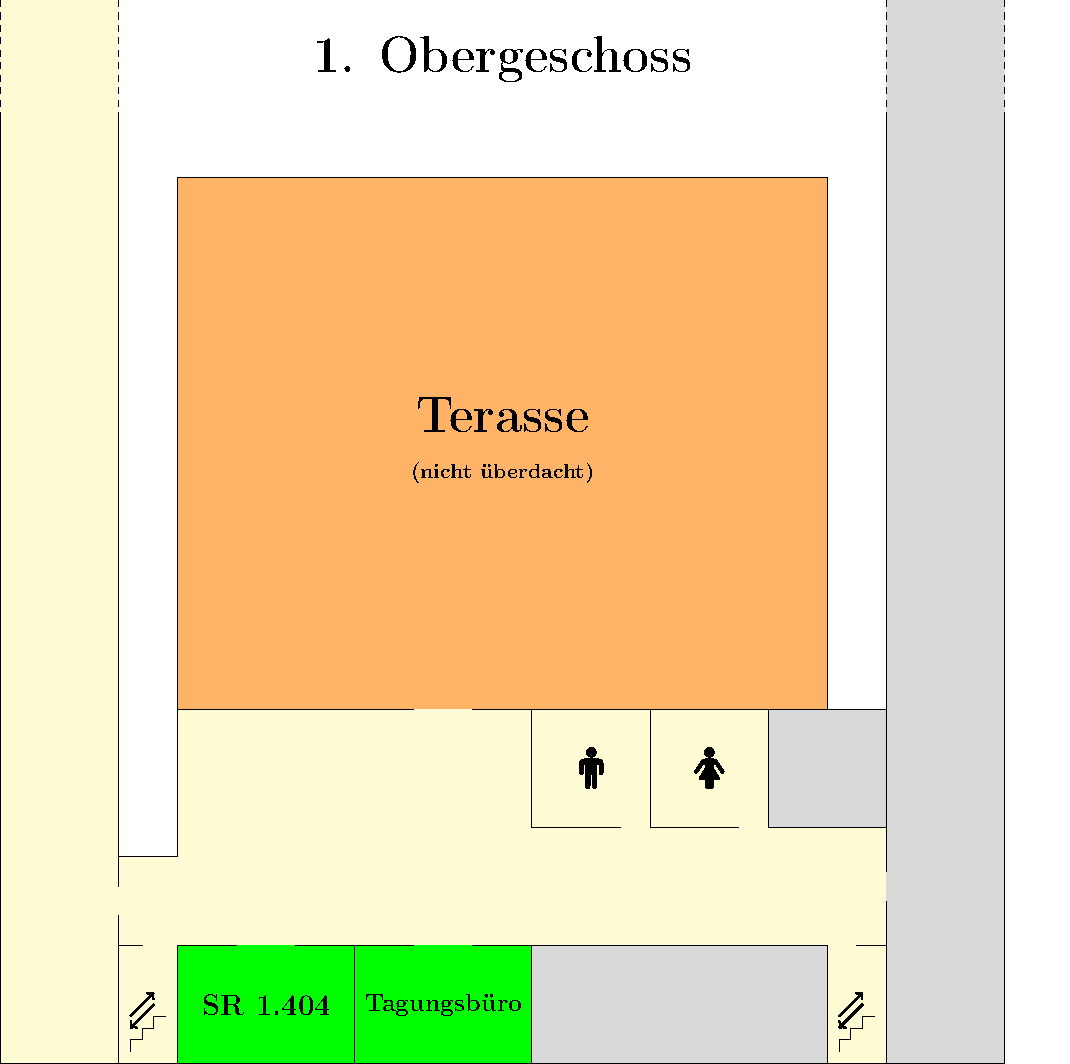
\includegraphics[width=\linewidth]{raumplan/og1}
\end{subfigure}
\end{figure}

\begin{figure}[H]
\centering
\begin{subfigure}[h]{0.62\textwidth}
\centering
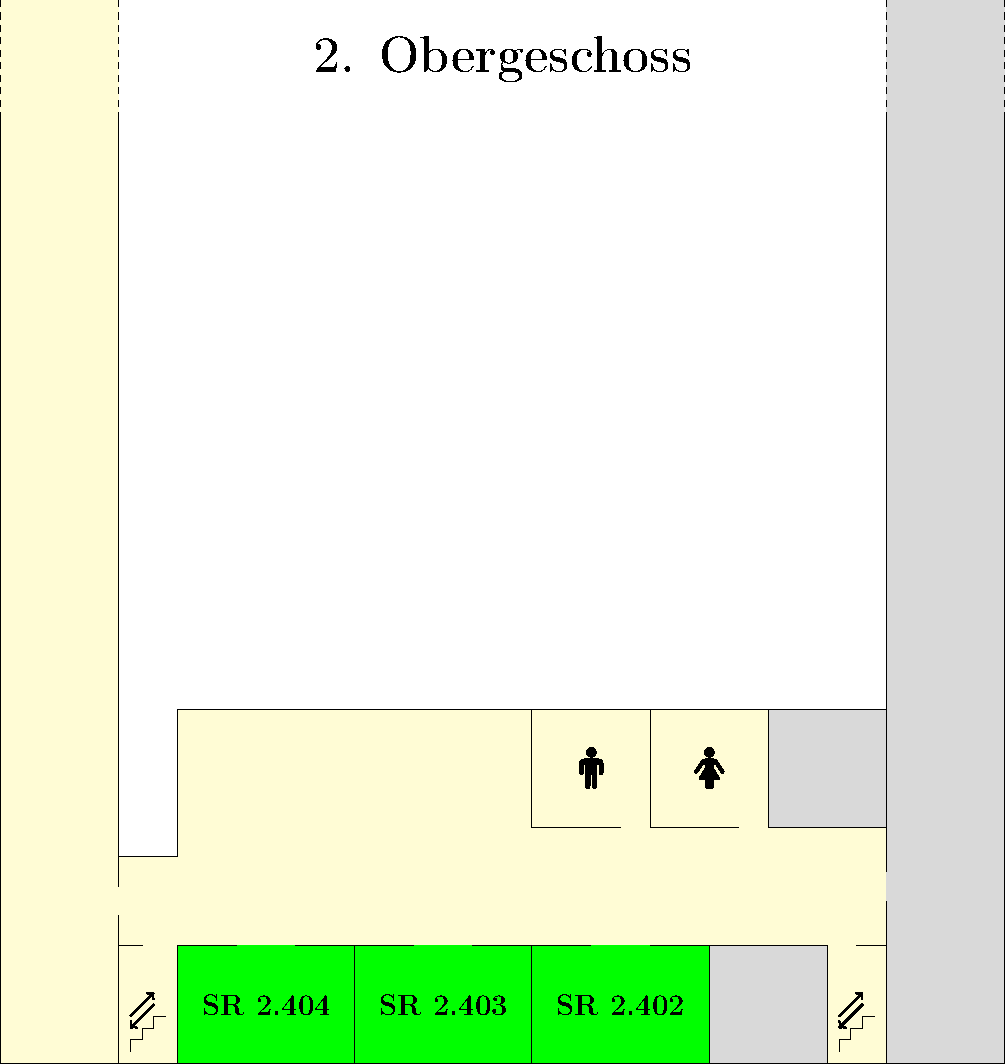
\includegraphics[width=\linewidth]{raumplan/og2}
\vspace*{5mm}
\end{subfigure}
\begin{subfigure}[h]{0.62\textwidth}
\centering
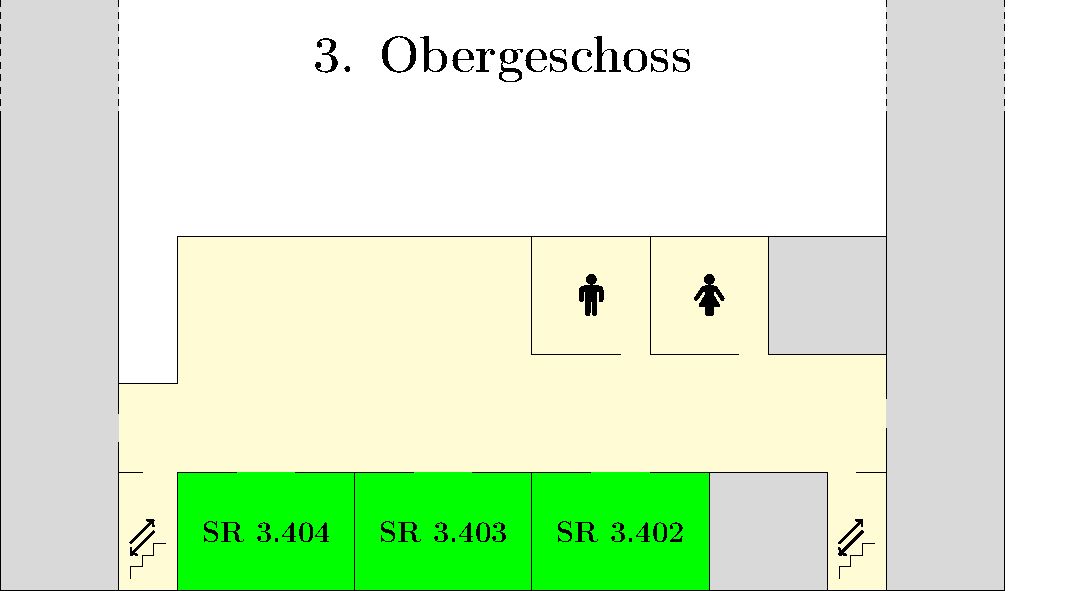
\includegraphics[width=\linewidth]{raumplan/og3}
\end{subfigure}
\end{figure}
